\documentclass[tikz, border=2mm]{standalone}
\usepackage{tikz}
\usetikzlibrary{arrows.meta, positioning}

\begin{document}
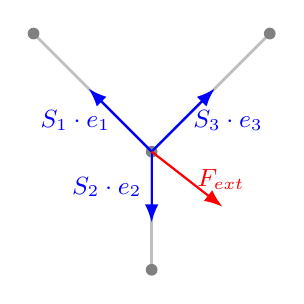
\begin{tikzpicture}[
    node_style/.style={circle, fill=gray, inner sep=1.5pt},
    force_style/.style={-Latex, thick, blue},
    label_style/.style={font=\small}
]

    \coordinate (node_i) at (0,0);
    \coordinate (node_1) at (1.5,1.5);
    \coordinate (node_2) at (-1.5,1.5);
    \coordinate (node_3) at (0,-1.5);

    % Rods
    \draw[line width=1pt, lightgray] (node_i) -- (node_1);
    \draw[line width=1pt, lightgray] (node_i) -- (node_2);
    \draw[line width=1pt, lightgray] (node_i) -- (node_3);

    % Nodes
    \node[node_style] at (node_i) {}; 
    \node[node_style] at (node_1) {}; 
    \node[node_style] at (node_2) {}; 
    \node[node_style] at (node_3) {}; 

    % Rod forces
    \draw[force_style] (node_i) -- node[left, label_style] {$S_1 \cdot e_1$} (-0.8, 0.8);
    \draw[force_style] (node_i) -- node[left, label_style] {$S_2 \cdot e_2$} (0, -0.9);
    \draw[force_style] (node_i) -- node[right, label_style] {$S_3 \cdot e_3$} (0.8, 0.8);

    % External force
    \draw[force_style, red] (node_i) -- node[right, label_style, red] {$F_{ext}$} (0.9, -0.7);

\end{tikzpicture}
\end{document}
